Este proyecto se alinea con varios Objetivos de Desarrollo Sostenible (ODS) de las Naciones Unidas. En concreto, se toma como referencia el marco de la \textit{EHUagenda 2030} de la UPV/EHU. Esta agenda, ``recoge la contribución de la UPV/EHU a 12 de los 17 ODS de la Agenda 2030, al que ha sumado el su compromiso con la diversidad lingüística y cultural a través del ODS 17+1'' [\hyperref[ch:bib]{1}]. A continuación, se detallan los objetivos específicos relacionados:

\begin{figure}[h]
    \centering
    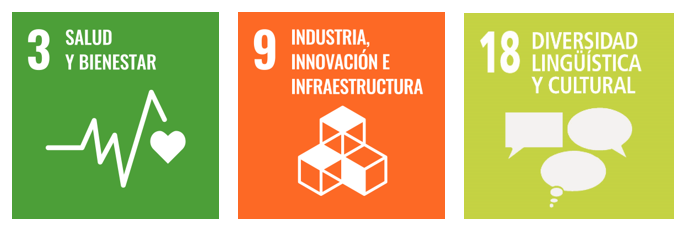
\includegraphics[width=0.6\textwidth]{figures/tres_ods_relacionadas.png}
    \caption{Los ODS alineados con este trabajo.}
\end{figure}

\begin{itemize}
    \item \textbf{ODS 3: Salud y Bienestar}. La música juega un papel importante en el bienestar emocional y mental. La capacidad que ofrece esta aplicación de mejorar la experiencia musical y permitir a los usuarios conectar más profundamente con su música contibuye positivamente a su bienestar general.
    \item \textbf{ODS 9: Industria, Innovación e Infraestructura}. Como este proyecto implica la utilización de tecnologías modernas como React, Next.js y Vercel durante el desarrollo, se fomenta la innovación tecnológica y se contribuye al desarrollo de infraestructuras digitales eficientes.
    \item \textbf{ODS 18 (17+1): Garantizar la diversidad lingüística y cultural}. Al permitir que los usuarios exploren y aprecien música de diferentes culturas y en diversos idiomas, se facilita la exposición a estas, fomentando así el entendimiento y la apreciación cultural, alineándose así con el objetivo 18 propuesto por la UPV/EHU.
\end{itemize}